
\documentclass[journal,12pt,onecolumn,draftclsnofoot]{ieeeconf}  % Comment this line out if you need a4paper

\usepackage{listings}
\usepackage{hyperref}
\usepackage{url}
\usepackage[pdftex]{graphicx}
\usepackage{amsfonts}
\usepackage{subfigure} 
\usepackage{algorithm}
%\usepackage{algorithmic}
\usepackage{amsmath}
\usepackage{bm}
\usepackage{algcompatible}
\usepackage{framed}
\usepackage{balance}

\usepackage{graphics} % for pdf, bitmapped graphics files
\usepackage{caption}
\usepackage{epsfig}
\usepackage{wrapfig}
\usepackage{breqn}
\newcommand{\myalpha}{\alpha_\rho}
\DeclareMathOperator*{\argmax}{arg\,max}

\pdfminorversion=4

\IEEEoverridecommandlockouts                              % This command is only needed if 
                                                          % you want to use the \thanks command
\overrideIEEEmargins                                      % Needed to meet printer requirements.

\author{Wenbo Xu, Wenwen Zhang, Yichi Zhang}

\title{
	EE 382C: Multicore Computing \protect\\
	\Large \bf Parallel GPU based Algorithms for Image Processing
}

\begin{document}
\maketitle
\thispagestyle{empty}
\pagestyle{empty}


\section{Abstract}
  

\section{Introduction}
Recently, the requirement for GPU (graphics processing unit) performance is increasing rapidly as well as the computation speed. As comparison, GPU computation speed can be several times faster than traditional CPU. Moreover, as the programmability and parallel processing emerge\cite{1}, GPU begins being used in some non-graphics applications, which is general-purpose computing on the GPU (GPGPU). To be more user-friendly, CUDA brings the C-like development 
environment and some CUDA extended libraries to programmers, which is based on industry-standard C/C++ and has straightforward APIs to manage devices, memory etc.

As an general use of GPU, Image processing algorithms are always computationally expensive, however, parallelize image processing algorithms can enhance the speed to a great extent, especially for large-scale images.

In this paper, we?

\section{Gaussian blur}
\subsection{Definition and Usage}
In image processing, a Gaussian blur (also known as Gaussian smoothing) is the result of blurring an image by a Gaussian function. It is a widely used effect in graphics software, typically to reduce image noise and reduce detail. 

Mathematically, the Gaussian blur is a type of image-blurring filter that uses a Gaussian function for calculating the transformation to apply to each pixel in the image.  For our implementation, we use a two-dimensions gaussian blur to filter each image pixel. The related two-dimensions gaussian function is the product of two such one-dimension function above, on in each dimention. 
  \[G(x) = \frac{1}{ \sqrt{2 \pi   \sigma ^{2} } } e^{ -\frac{ x^{2} +  y^{2}}{2  \sigma ^{2} }}\]
 Variable $x$ is the distance from the origin in the horizontal axis, $y$ is the distance from the origin in the vertical axis, and $\sigma$ is the standard deviation of the Gaussian distribution. A convolution matrix is built with values generated by this distribution.  
 To have a better view of the powerfulness of parallel computing, we did a comparison experiment, which is comprised with two implementations of Gaussian blur. One is sequential implementation and the other is parallel implementation. 

\subsection{Sequential  Implementation}
There are four steps of the sequential implementation. The first step is preprocess, which is responsible for reading image file and store it as Image class. The second step is to generate a gaussian filter, a matrix, based on parameters, like the standard deviation,  passed from users. The next step is to traverse each pixel in the image object and compute the values of a given pixel in the output image by multiplying each kernel value by the corresponding input image pixel values. The final step is to generate an image file from those new pixel values.

\subsection{Parallel  Implementation}
In this chapter, we implemented a normal parallel version gaussian blurring based on CUDA. In the following chapter, we optimized this implementation in several ways.  Firstly, we read the image file and generate filter matrix. Then we need to copy the image into device memory. Each pixel is combined with three channels, $r$, $g$ and $b$.  They should be separated and be gaussian blurred separately. So we use $cudaMemcpy2D$ to copy each channel of image file from host to device. Then we start the kernel three times and do gaussian blurring to each channel per time.  At last, we copy three blurred channels from device to host and save them into an image fileThis process is described in details with the Fig.1 and Fig.2.


\begin{figure}[h]
	\centering\includegraphics[width=85mm,height=92mm]{ImageProcessingCuda.png}
	\caption{Diagram for Parallel Image Processing}
	\label{parallel}
\end{figure}

\begin{figure}[htbp]
\begin{center}
\fbox {
\begin{minipage}  {\textwidth}\sf
\begin{tabbing}
x\=xx\=xx\=xx\=xx\=xx\= \kill

{\bf compute} $thread2DPos$ and $thread1DPos$\\
\> $thread2DPos.x = blockIdx.x*blockDim.x  + threadIdx.x$\\
\>$thread2DPos.y = blockIdx.y*blockDim.y+ threadIdx.y$ \\
\>$thread1DPos = thread2DPos.y*numCols + threadIdx.x$
\\
\>{\bf set} $output$ $image$ $pixel$ to accumulator \\



\end{tabbing}
\end{minipage}
}
\end{center}
  \caption{Pseudo-code for Gaussian Blur per Thread}
\end{figure}


\section{Optimization}

\subsection{Pageable vs. Pinned Memory}
Host data allocations are pageable by default, which means can be paged in/out between RAM and disk. However, GPU cannot access data directly from pageable memory, but from pinned memory, which means page-locked. Hence, whenever a data transfer is invoked on pageable memory, the CUDA driver has to allocate a temporary pinned memory array to copy host data and then transfer it to the device. \par
\begin{figure}[h]
	\centering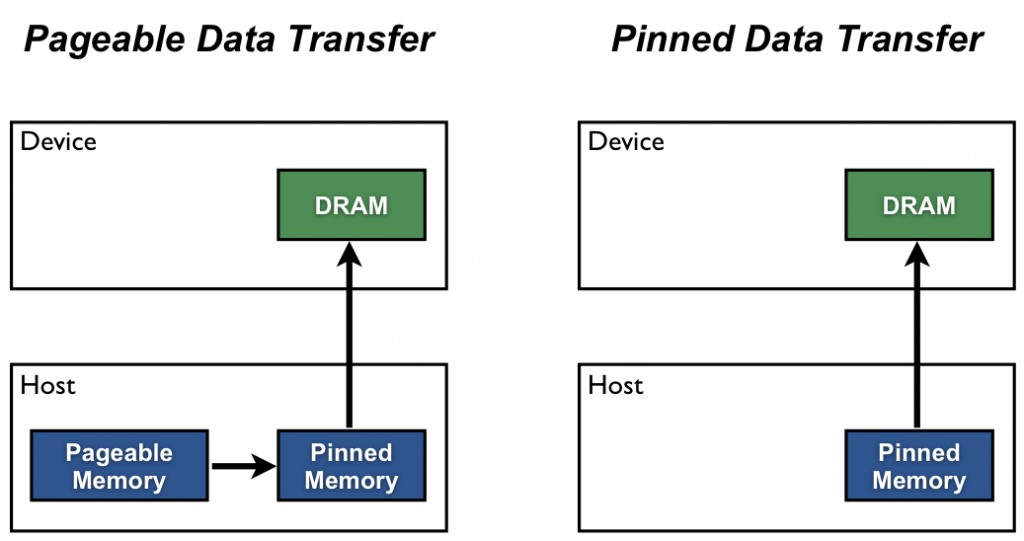
\includegraphics[width=120mm]{pinned.jpg}
	\caption{CUDA data transfer.\cite{Mark}}
	\label{CUDA data transfer.}
\end{figure}
We can avoid the cost of this overhead by using pinned memory for host instead of pageable memory. In this case, we use \textit{cudaMallocHost()} and \textit{cudaFreeHost()}. Compare to the \textit{malloc()} and \textit{free()}, \textit{cudaMallocHost()} and \textit{cudaFreeHost()} are more expensive with additional overheads. Then, the question has been raised about how should we made the tradeoff. According to figure below, pinned memory is faster when the size of data to be transfered is larger than 16MB.  	\cite{Trade_off}\par
\begin{figure}[h]
 	\centering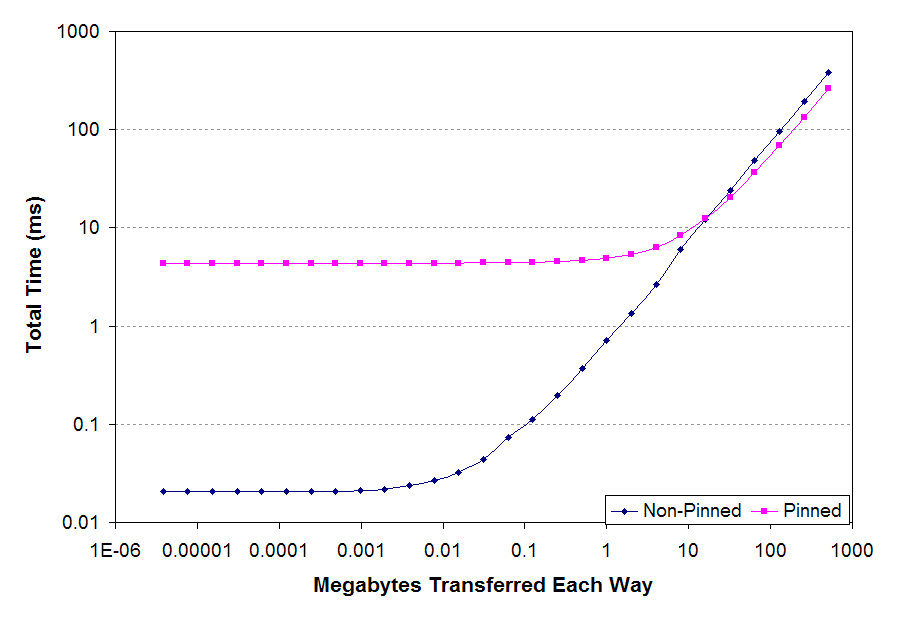
\includegraphics[width=120mm]{pinned_trade_off.png}
 	\caption{Time required to allocate, transfer to the GPU, transfer back to the CPU, and deallocate pinned and non-pinned memory.\cite{Trade_off}}
 	\label{Time required to allocate, transfer to the GPU, transfer back to the CPU, and deallocate pinned and non-pinned memory.}
\end{figure}
This doesn't mean we should never use pinned memory when the amount of data to be transfered is less than 16MB. One example is the asynchronous memory copy, \textit{cudaMemcpyAsync()} can be used only with pinned memory. The details of how asynchronous memory copy would be used to improve the efficiency will be discussed in next section.

\subsection{Streams}
A stream is defined as a sequence of operations in that execute in issue-order on the GPU. CUDA operations, which are kernal operations and memory operations, in same streams are ordered and in different streams can overlap. By default, all operations are in default stream. The following code is used to specify which stream the operation is in. \par

The figure below illustrate the execution time line for three different scenarios. The top time line shows time line without use of streams, which all operations executes in sequential order. The time line in the middle shows the use of streams on hardware has only one copy engine. The performance improvement is significant. The bottom time line shows the time line for hardware has two copy engines. With two copy engines, the HD (Host to Device memory transfer) and the DH (Device to Host memory transfer) can execute concurrently without arbitrating for the same hardware. \par 
For memory copies, \textit{cudaMemcpyAsync()} is used. As described in last section, we have to allocate pinned memory using \textit{cudaMallocHost()}. This method place transfer into the stream and returns immediately. It is upto device to schedule streams when the corresponding resources are free. It allows us to put memory transfer operations and kernel operations into the stream the same time and allow them to run concurrently.\cite{Stream} \par
\begin{figure}[h]
	\centering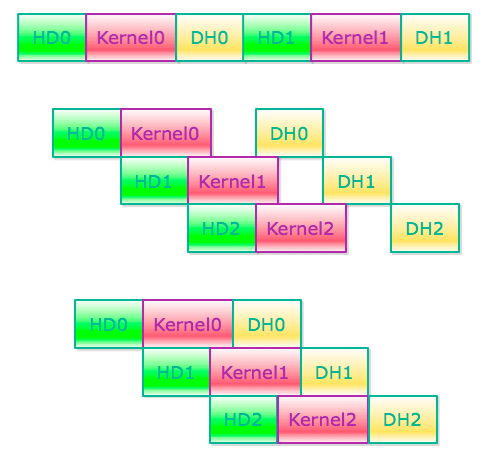
\includegraphics[width=120mm]{concurrent.png}
	\caption{Top: all operation in default stream. Mid: concurrent streams with one copy engine. Bottom: concurrent streams with two copy engine.}
	\label{concurrent}
\end{figure}

\section{Results}
Both CPU and GPU implementations was running on the TACC Stampede Supercomputer. The CPU is Intel® Xeon® E5-2680 2.7GHz Processors. And the GPU is NVIDIA K20 with 5120 MB GDDR5 memory and 2 copy engines. \par
The command line tool, nvprof, and the Nvidia Visual Profiler are used to profile the performance of our implementation. And the results are shown in the table below.

\section{Conclusion} 

\bibliographystyle{abbrv}
\begin{thebibliography}{9}
\bibitem{1}
WU En Hua , ?State of the Art and Future Challenge on General 
Purpose Computation by Graphics Processing Unit?, Journal of 
Software, vol. 15, no. 10, 2004,pp.1493~1504.

\bibitem{Mark} 
Harries, M. (2012, December). How to Optimize Data Transfers in CUDA C/C++. Retrieved from https://devblogs.nvidia.com/parallelforall/how-optimize-data-transfers-cuda-cc/
	
\bibitem{Trade_off} 
Boyer, M. Choosing Between Pinned and Non-Pinned Memory. Retrieved from https://www.cs.virginia.edu/~mwb7w/cuda_support/pinned_tradeoff.html
	
\bibitem{Stream} 
Harries, M. (2012, December). How to Overlap Data Transfers in CUDA C/C++. Retrieved from https://devblogs.nvidia.com/parallelforall/how-overlap-data-transfers-cuda-cc/
	

\end{thebibliography}

\end{document}
